% !TEX root = ../main.tex
\chapter{Fun with cats}
\begin{figure}[tb]
	\begin{subfigure}{.3\textwidth}
		\centering
		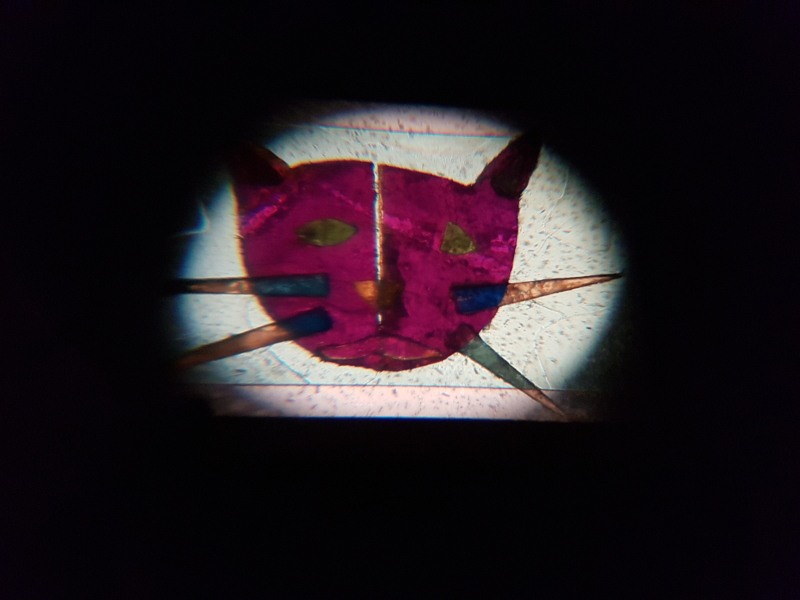
\includegraphics[height=.8\linewidth]{./img/cat1.jpg}
		\label{subfig:cata}
	\end{subfigure}
	$\quad$
	\begin{subfigure}{.3\textwidth}
		\centering
		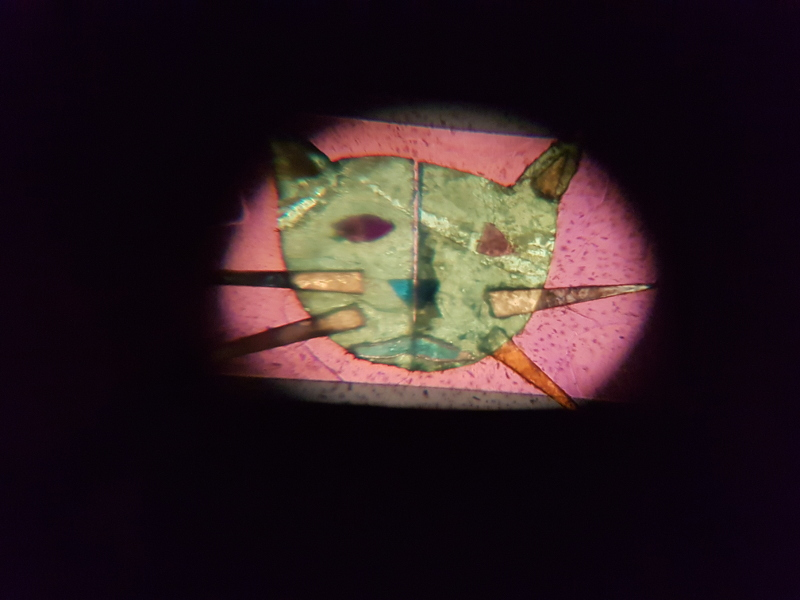
\includegraphics[height=.8\linewidth]{./img/cat2.jpg}
		\label{subfig:catb}
	\end{subfigure}
	$\quad$
	\begin{subfigure}{.3\textwidth}
		\centering
		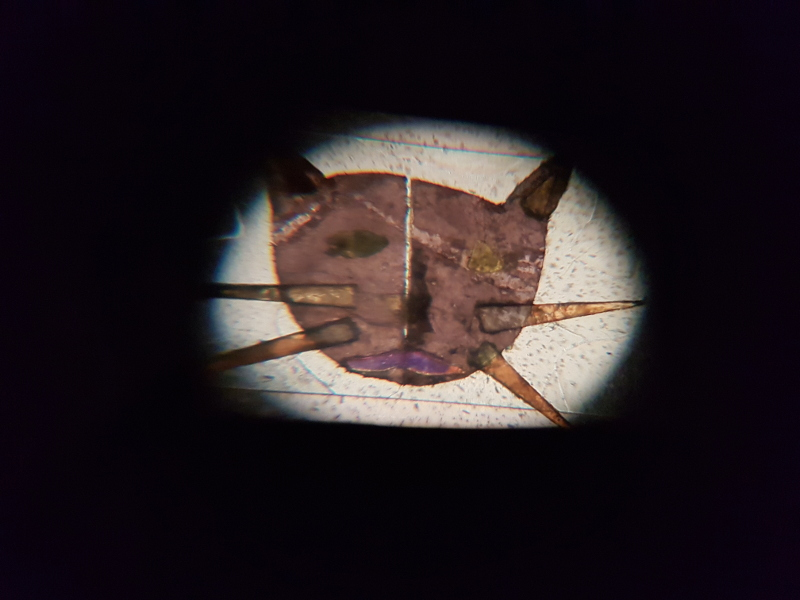
\includegraphics[height=.8\linewidth]{./img/cat3.jpg}
		\label{subfig:catc}
	\end{subfigure}
	\caption[Doppelbrechung von polychromatischem Licht]{Messungen des doppelgebrochenen Lichtes am Klebefilmbild}
	\label{fig:cats_not_the_musical}
\end{figure}
Nach Entfernung des Bandpassfilters wird ein Klebefilmmotiv anstelle des Glimmerplättchens in den Strahlengang gebracht.
Auch der Klebefilm ist doppelbrechend, weshalb das Licht nach diesem elliptisch polarisiert ist.
Da die Doppelbrechung abhängig von der Wellenlänge des Lichtes ist, werden mit der Drehung des Analysators verschiedene Wellenlängen des Lichtes stärker oder schwächer durchgelassen.
Daher ändern sich die Farben des Bildes je nach Stellung des Analysators.
\autoref{fig:cats_not_the_musical} zeigt ein Katzenmotiv für verschiedene Einstellungen des Analysators.
Bemerkenswert ist, dass die Farben in \autoref{subfig:cata} und \autoref{subfig:catb} zueinander komplementär sind und zwischen den Bildern eine Winkelverschiebung des Analysators von $\SI{45}{\degree}$ besteht.
